\chapter{Project 1: Multi-Currency Consumer}

\section{Introduction}
When I was first presented with this task, I thought it would be fairly simple as on the surface, it seemed like simply getting what type of multicurrency change is being made and then just adding the field to the database. Once I had gotten started, it became much more complex and required multiple steps and code refactors whilst the project was being built. \\ For example, when a user makes a change to a multicurrency to their HubSpot portal, the consumer would then process what type of change was made (addition/deletion being the only two the conusmer was concerned with) and from there, the consume would create a a HubSpot standardized field and place it into the database for the user alongside other fields such as the label to be displayed in the UI in the case of an addition and in the case of a deletion, the consumer would remove the corresponding fields from the database. \newline \\ This change seemed pretty simple but there's multiple hidden requirements that aren't immediately obvious. For instance, what should be done for all the multicurrencies that are already in a user's portal? What should be in the case where a user doesn't yet have any multicurrencies in their portal and decides to add one? How are calls to/from the database to be handled? Questions like these and many others needed to be answered and dealt with before and during the coding process. \\ Luckily for me, my team had started some of the necessary work making it easier for me to get to coding. For instance, my team already had created the Kafka producer and set up much of the infrastructure so I just had to work with it to do complete this task.

\section{Design Approach and Architecture}
To complete this task, I split the overall task into multiple subtasks to be completed:
\begin{itemize}
\item Standardized Multicurrency labels and fields Generator
\item Build Kafka Consumer
\begin{itemize}
\item Filter Kafka message into Add/Delete
\item Pre-build request body for processed message
\item Send request
\end{itemize}
\item Create Internal Endpoints for adding/deleting multicurrencies
\item Build Wrappers for hitting endpoints to be used by Kafka Consumer
\end{itemize}

I went with a top down approach initially when defining each of the individual components and fleshing out components as I went along. I decided to use this as I was sure there may be some hidden requirements that may arise during the coding process. Also, the top down approach to software engineering is much more requirements driven and was more in-line with clean code practices as I could avoid writing code I may not need. For some of the individual components, I did go with more of a bottom up approach like the kafka consumer, as this consumer could be reused for something elsewhere with some changes to the functionality. \newline \\ For the overall architecture, I went with one of the more common design patterns, the \textbf{Model-View-Controller (MVC)} system. I went with MVC due to the scalability it provides alongside the support for asynchronous techniques like Apache Kafka which is a major framework in use at HubSpot.

\subsection{Model-View-Controller (MVC)}
MVC is a common architecture pattern used in web based applications. MVC separates out the layers of business logic and data interactions(model) from the presentation(view) and intermediary between the two layers(controller). This pattern is so popular as it decouples each of the major aspects of the design from each other and is also highly scalable due to how modular the design is.


\subsubsection{Model}
The data and business logic of the application are wrapped in the model layer.
It's frequently made up of a number of interconnected domain objects.
The models represent the nouns or entities in the system, such as user or order, and interact with any of the other layers of the system.  
\newline The model layer, on the other hand, includes not just models but also validators, methodologies, and any other element that directly affects or distorts the underlying data of the application. \newline \\ 
Each model has a user interface that reflects the logical functions that can be performed on the data it represents.
An illustration of the capabilities contained in an application's model layer: A \textit{FullName} method on a User class returns a merger of the first and last names associated with the user it depicts. The same object also has an \textit{UpdateName} function that updates the corresponding name in the database. The same object could then use a Validator instance to make sure none of the fields are empty before being placed into the database.  \newline \\
The model Layer often utilises some form of \textbf{Object Relational Mapping},  which is a layer of abstraction which is designed to transfer data from the the scalar values used in database storage to the objects used in object orientated programming languages and vice versa.  While a traditonal SQL database is used in many instances,  noSQL databases and/or web services that perform some sort of data persistence could be used as the database layer instead. 
\newline In many versions of the model class,  a set of static methods which utilise the ORM to search for and instantiate instances of the model.
\subsubsection{View}
The 'View' layer is responsible for the visual layer of the model.  This represents the graphical user interface a user may interact with. Views perform as the output of the system, whereby data from the model is represented.  In many MVC architectures,  the view is sensitive to changes in the data held in the model and hence self updates to reflect any new changes in the data.  The view itself does not transformations or alterations of the data itself,  it just acts as thin layer between the model and the controller.  Data from the user may be inputed in the view layer but is ultimately sent to the controller to be dealt with.
\subsubsection{Controller}
The controller layer is primarily responsible for processing user input.  A controller normally has a 1-to-1 relationship with a view or a 1-to-many relationship with a series of views.  When a user inputs data via an interface in the view layer,  this triggers an event to occur which is dealt with by the controller layer. The controller layer could for instance instruct the view layer to resize itself if a user resizes the size of the input window.  Another example is to update the data in the model and hence update the view layer if a user inputs new data into the view layer initially.  Controllers have permissions to frequently access the model layer and re-construct and transform the data in that layer.

\begin{figure}[ht]
  \centering
  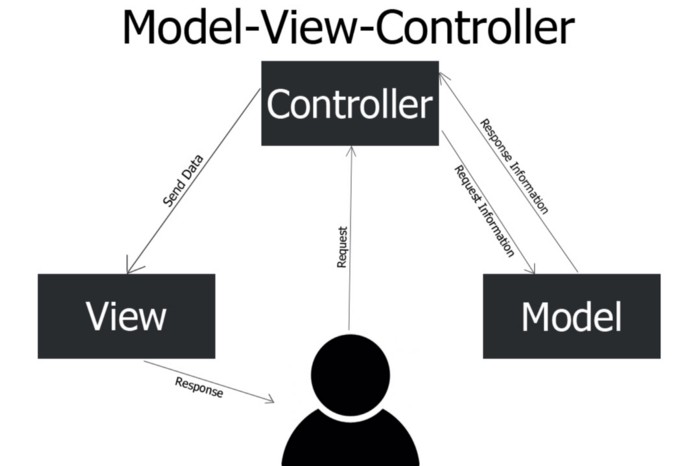
\includegraphics[scale=0.35]{multicurrency/mvc.jpg}
  \caption{Model-View-Controller overview}
\end{figure}


\section{Implementation}
For the implementation of this task, it was split into multiple sub-tasks with each part being tested individually before the next part was created.
\subsection{Standardized Labels and Fields Generator}

The first task I worked on was creating a function that would take in some multicurrency and then convert it to a HubSpot standardized field. \newline For example,  the function would take in a currency like \textit{USD} and then return it in the form \textit{hs\_external\_price\_USD}.  \newline Initially this change was simple to write as it required only the name of the currency that is being used to create the field according to the ISO 4217 standard.  \newline \\ As work progressed on this function,  it was refactored slightly and given some more utility to be able to generate more fields that had to do with multicurrencies.  A function to create the internal version of the fields was also created alongside the labels that would be displayed in the UI on the page in a users portal where multicurrencies would be managed.  \newline This task took some time to get to production as there was a number of comments on the pull requests that needed to be implemented as it was my first major pr.  This change showed me how to write code according to the level that's expected at HubSpot.

\subsubsection{Problems} 
The major problem that arose was that for some 3rd party developers didn't use the ISO 4217 standard for the currencies so matching them in the syncing engine wasn't possible.  \newline To get around this issue,  we first of all had to check if the inputted multicurrency was ISO 4217 compliant and then from there would generate the field.  Any input data that was not compliant would then return an error.

\subsubsection{Testing}
In terms of testing for this change,  I wrote a series of unit tests to test the different expected behaviours of this change.  The tests were written in advance of the code being written as at HubSpot test-driven development is a big thing and is greatly encouraged. 

\subsection{Kafka Consumer}
The next task I worked on was creating kafka consumer to consume messages from the kafka producer queue. This was a much larger task than the previous task so I split it up into smaller pieces to make the task more manageable. This aspect of the task would fall into the ''Controller'' layer of the MVC framework as all data operations are performed here before being sent to the database or 'Model'

\subsubsection{Building The Base Consumer}
The base kafka consumer was constructed from an interface for building kafka consumers that was already pre-created. The consumer was subscribed to a topic that was responsible to publish messages concerning multicurrency updates from a producer. When a message gets published to the queue, the kafka consumer would then grab the message from the queue and then process it accordingly. 

\subsubsection{Filtering Kafka Messages}
The next major part of the consumer I wrote was to grab the type of request in the message and from there, process the message accordingly. To process the message, I used a switch statement to filter the data based off the type in the message body. The currency being updated in question is then also extracted from the message body.

\subsection{Pre-building The Request Body}
Once the major aspects of the request has been collected from the message body, the request body is then created. The label's, standardized fields and such are all created here.

\subsubsection{Sending the Request}
Once all the previous steps have been completed, the request is then sent to the corresponding internal endpoint, using the previously built request body. 

\subsubsection{Problems}
One of the major problems in creating this consumer was figuring out how to prevent messages being processed twice. Luckily, kafka has numerous guarantees that ensure that each message is processed exactly once making this a none issue. Another issue was figuring out how to scale this to work on a large scale. To solve this issue, kafka enables multiple kafka workers to be subscribed to a topic so more workers can be spun up as necessary or killed as traffic changes. 

\subsubsection{Testing}
To test this change, a number of integration tests were written to make sure each of the core components interacted with each other as necessary. As each of the individual components do different things, unit testing the overall system wasn't possible. Each of the individual components were unit tested as necessary. One bug that was encountered in testing was getting the correct multicurrency field from the topic. To fix this issue, I had to re-parse the data given from the topic into ISO 4217 compliant fields.

\subsection{Endpoints}
The next major component that needed to be written was the internal endpoints that would hit the database and update the data in there. This would compromise part of the 'Model' aspect of the MVC framework as it's responsible for framework operations. The endpoints needed to be internal as we didn't want to expose them to external developers and also it allowed us to use the '@internal' annotation to allow it to be secure by using Oauth. \newline \\ To create the endpoints, a path was first defined for both the add and delete endpoints in seperate functions. From here, we could then hit the database directly using some ORM methods. This component didn't take much time to create as it was a relatively easy aspect to code as it was basically a partial implementation of a REST api. \newline \\ The endpoints that were created were  \begin{itemize}
\item An 'Add' endpoint to create a multicurrency field mapping in the database
\item A 'Delete' endpoint to remove multicurrency field mappings in the database
\end{itemize}

\subsubsection{Problems}
One issue that I faced writing this was dealing with verification as I had initially planned on creating an open endpoint and hitting it as necessary. But I kept getting errors due to verification due to the fact I was trying to hit internal database's via external calls. To solve this, I made the endpoints internal which enabled stopped these errors from appearing as Oauth was used for verification automatically so I didn't need to worry about security.

\subsubsection{Testing}
To test this change, I did some integration testing instead of End-to-End testing as external users wouldn't have access to this endpoint so all that mattered was that it performed according to the parameters we expected. I did some asserts on the expected response from the endpoints, and mocked out the calls to the database as this was beyond the scope of the test. 


\subsection{Wrappers for Endpoints}
The final part to complete this task was to write some wrappers around the endpoints defined above.  Whilst the endpoints could be accessed without wrappers,  to make the code cleaner,  more maintainable and also more reusable,  creating api wrappers was the best choice.  \newline
This code addition was also rather small,  all that was necessary was to create functions that would take in the request from the kafka consumer and then send them to endpoint where they'd be dealt with.  These functions acted as part of the 'Controller' aspect of the MVC architecture.  \newline \\ For testing and problems encountered, since this wasn't a huge change, no real problems were encountered whilst writing these wrappers. 

\section{Evaluation and Testing}
Once all the parts of the consumer had been created,  testing the entire flow of the system became top priority.  Whilst each of the individual parts were unit tested and integration tested,  an end-to-end test of the entire system could only be done when the entire thing was assembled.  \newline \\ To test the entire system,  using Orion,  a branch deploy was done of the code base including this consumer to the staging environment.  Next,  all active Kafka consumers subscribed to this topic in staging were temporarily paused to test this change to prevent a flood of errors being sent in case the change had some bugs.  Finally,  testing was done using a test portal. \newline To begin testing,  I started with testing adding new multicurrencies.  To evaluate if the change worked,  I searched the logs for https requests and checked if they were going to the correct services.  Finally,  I checked the database to see if the new fields were added to the test portal.

\subsection{Problems encountered}
One issue I found while testing was I saw requests were not going to the correct services but were ending up somewhere completely different.  I initally checked my code to debug it but I couldn't seem to figure out what was going wrong.  Next I ran the kafka worker locally to find out what was wrong as I could debug it step by step as new requests came in, but again I couldn't figure out what was wrong.  I finally asked my Team Lead for assistance,  it turned out that because I was testing in Staging,  the route requests take is slightly different as there are 2 streams in Production to deal with all the traffic while in Staging there's only 1 as it's just for testing.  I was expecting the route of traffic to match Production but it turned out the testing was working as intended,  my assumptions were just wrong. 
\section{Analysis and Possible Changes}
